\section{Defining Tap Points}
\label{sec:tapdef}

\begin{figure}[t]
\begin{center}
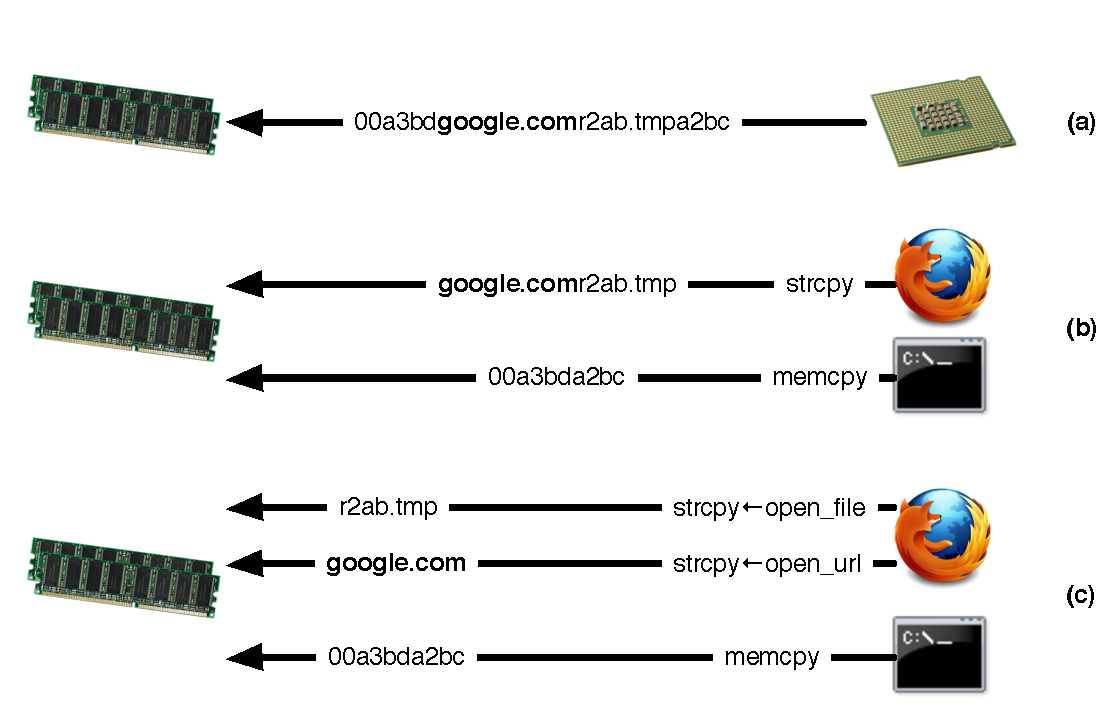
\includegraphics[width=3.2in]{tappoint.pdf}
\end{center}
\caption{Three different ways of defining a tap point: (a) as a single
stream of information from the CPU to RAM ; (b) split up according to
program and location within program ; (c) split up according to program,
location within program, and calling context.}
\label{fig:tappoint}
\end{figure}

At the heart of our approach is an abstraction on top of memory accesses
made by the CPU, the \emph{tap point}. A tap point is a point in a
system at which we wish to capture a series of memory accesses for
introspection purposes; however, the exact definition of ``a point in a
system'' will make a great deal of difference in how effective our
approach can be.

A naive approach to defining tap points would be to simply group memory
accesses by the program counter that made them (e.g., EIP/RIP on x86 and
R15 on ARM). This approach fails in two common cases: first, memory
accesses made by bulk copy functions, such as \texttt{memcpy} and
\texttt{strcpy}, would all be grouped together, which would commingle
data from different parts of the program into the same tap point. In
addition, looking only at the program counter would conflate accesses
from different programs.

Instead, we define tap points as the triple
\[ (caller, program\_counter, address\_space) \]
Including the caller and the address space (the \texttt{CR3} register on
x86, and the \texttt{CP15 c2} register on ARM) separates out memory
accesses into streams that should, in general contain the same type of
data.\footnote{Making use of tap points defined this way in the real
world is slightly more difficult, since a program's address space will
differ and its code may be relocated by ASLR. These complications can be
overcome with a minor amount of engineering, however.} Figure
\ref{fig:tappoint} shows the effect of choosing various definitions of a
tap point when looking for the place where the browser writes the URL
entered by the user (``google.com''). At the coarsest granularity (a),
one can simply look at all writes from the CPU to RAM; however, the
desired information is buried among reams of irrelevant data.
Separating out tap points by program and program counter (b) is better,
but still combines uses of \texttt{strcpy} that contain different
information --- in this case, a filename and a URL. By including the
calling context (c), we can finally obtain a tap point that contains
just the desired information.

It is possible that some tap points may require deeper information about
the calling context (for example, if an application has its own wrapper
around \texttt{memcpy}), but in practice we have found that just one
level of calling context is usually sufficient. In addition, because TZB
uses a whole-system emulator that can watch every call and return, we
can obtain the call stack to an arbitrary depth for any tap point. This
makes it easy to add extra context for a given tap point, if it is found
that doing so separates out the desired information. Examples of tap
points that require more than one level of callstack information are
given in Sections \ref{sec:eval:subsec:ssl} and
\ref{sec:eval:subsec:file}.

Conversely, one might wonder whether this definition of a tap point may
split up data that should logically be kept together. To mitigate this
problem case, we introduce the idea of \emph{correlated tap points}: we
can run a pass over the recorded execution that notices when two tap
points write to adjacent locations in memory in a short period of time
(currently 5 memory accesses). The idea is that these tap points may be
more usefully considered jointly; for example, a single data structure
may have its fields set by successive writes. These writes would come
from different program counters, and hence would be split into different
tap points, but it may be more useful to examine the data structure as a
whole. By noticing this correlation we can analyze the data from the
combined tap point.
